%
% main.tex - a typical phil presentation
%
% Copyright (c) 2011, Phil Maker
% 
% All rights reserved.
%    
\documentclass{beamer}
%\documentclass[a4paper,handout]{beamer}
%\usepackage{pgfpages}
%\pgfpagesuselayout{4 on 1}[a4paper,border shrink=5mm]
\mode<presentation>{\usetheme{Pjm}}
\usepackage{graphics}
\usepackage{fancyvrb}
\newenvironment{code}
{\Verbatim[fontfamily=courier,%
numbers=right,stepnumber=5,%
firstnumber=\the\inputlineno]}%
{\endVerbatim}

\usepackage[english]{babel}
\usepackage[latin1]{inputenc}
\usepackage{hyperref}
\definecolor{links}{HTML}{2A1B81}
\hypersetup{
  pdftitle = {PV Diesel 101},
  pdfsubject = {PV Diesel}
  pdfkeywords = {Energy, Renewables, Powerwater, Phil Maker},
  pdfauthor = {\textcopyright\ Phil Maker, ..},
  pdfcreator = {\LaTeX\ with package \flqq hyperref \frqq},
  colorlinks,linkcolor=,urlcolor=links
}

# select various versions
\usepacakge{comment}
\excludecomment{nt-solar-concentrators}
\includecomment{nt-tkln}


\title{PV Diesel 101}
\author{Phil Maker
  \href{mailto:philip.maker@gmail.com}{\texttt{<philip.maker@gmail.com>}}
}
\institute{ACEP/Powerwater Remote Operations}
\date{March 2014}
\logo{
\includegraphics[height=0.7cm]{logo.jpg}}
\begin{document}

\begin{frame}
  \maketitle
  \vspace{-1.2cm}
  \begin{abstract}
    \small A review of energy storage in hybrid systems in Remote Australia
    including the messy bits (well a wee bit at least).
  \end{abstract}
\end{frame}

\section{Overview}
\begin{frame}\frametitle{Where: Australia}
\begin{columns}
\begin{column}{7cm}
  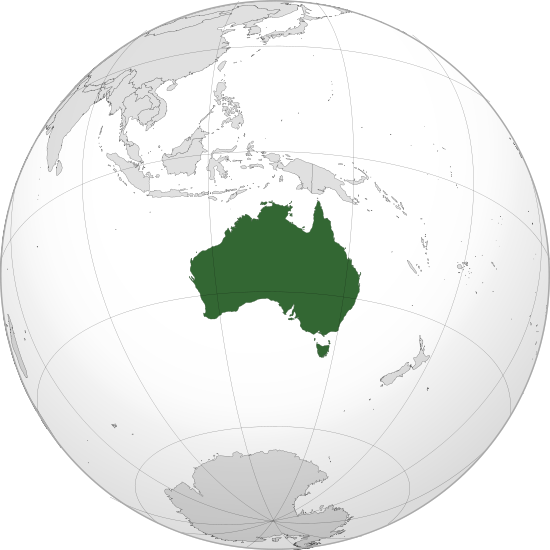
\includegraphics[width=6cm]{AU.png}
\end{column}
\begin{column}{5cm}\it
\href{http://www.kiplingsociety.co.uk/poems_serving.htm}{``I keep six honest serving men,
They taught me all I knew,
Their names are What and Why and When
And How and Where and Who.''} -- \href{http://en.wikipedia.org/Rudyard_Kipling}{Kipling}
\pause
\begin{itemize}
\item Energy storage in NT/WA.\pause
\item And the conniptions and kerfuffles (see handbook).\pause
\item Feel free to interrupt or redirect me.
\end{itemize}
\end{column}
\end{columns}
\end{frame}

\section{Northern Territory}
\begin{frame}\frametitle{Northern Territory/\href{http://www.powerwater.com.au}{Powerwater}}
\begin{columns}
\begin{column}{5cm}
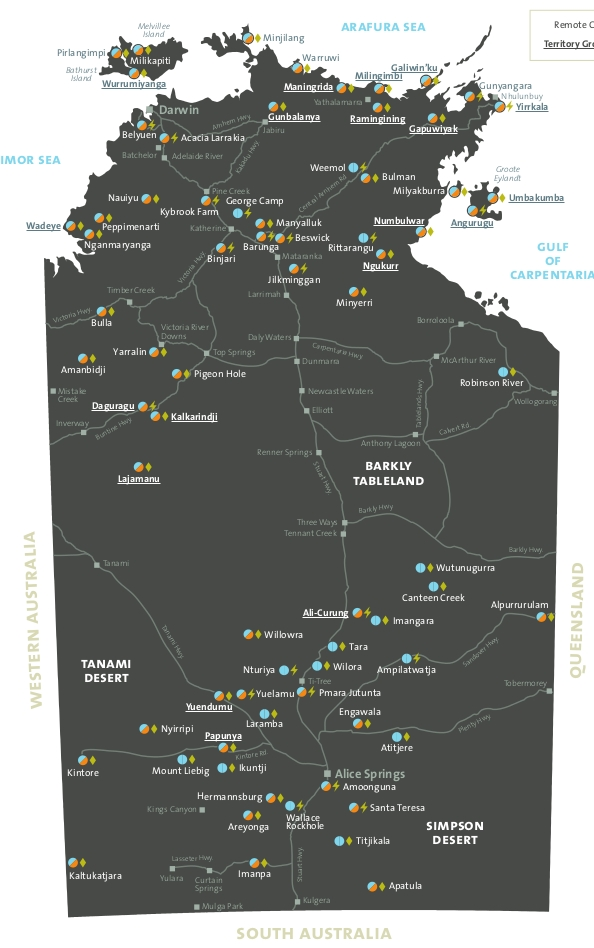
\includegraphics[width=5cm]{PW_map_section_A4.jpg}
\end{column}
\begin{column}{6cm}
  \begin{itemize}
  \item Early \href{http://www.sma.de/en.html}{SMA} systems for delaying gen switch up (20y lifetime).
  \item Small ($\approx$ 50kW) PV/Wind systems.
  \item Concentrated PV with limited smoothing.
  \item \href{http://www.epuron.com.au/project/tkln}{Ti Tree, Kalkarindji and Lake Nash} ($\approx$ 1MW total PV, 80\%
    peak penetration).
  \item \href{http://www.powerwater.com.au/solardiesel}{ASIM and Solar Diesel Handbook.}
  \item Medium Pen Rollout.
  \item High Pen Diesel off systems.
  \end{itemize}
\end{column}
\end{columns}
\end{frame}

\section{So..}
\begin{frame}\frametitle{So what!}
  \begin{itemize}
  \item Share our lessons learnt in a frank fashion.\pause
  \item Chemistry is difficult.\pause
  \item Its not just the technology.\pause
  \item Don't look at the problem just from your interests, e.g. in my case
    control systems.\pause
  \item Try to replicate projects/share risks,\pause
    particularly with remote battery chemistry.
  \end{itemize}

\vfill
  \begin{quote}
``Learning is not compulsory... \par\pause
neither is survival'' -- W. Edwards Deming
  \end{quote}
\end{frame}
\end{document}

